The last study is conducted to capture the impact on the 
performance of Lazy Shadowing brought by 
collocation overhead. We re-model the speed of shadows as $\sigma_s^b=\frac{1}{\alpha^{1.5}}$ to simulate the 
effect of memory thrashing and context switch. 
Figure~\ref{fig:comp_vary_fail_speed} shows the impact of collocation overhead on expected energy consumption for Lazy Shadowing with $\alpha=5$, with all the values normalized to that of process replication. The results for other values of $\alpha$ have similar behavior and thus are not shown. As expected, energy consumption is penalized because
of slowing down of the shadows. It is surprising, however, that the impact is negligible, with the largest difference being 4.4\%. The reason is that Lazy Shadowing can take advantage of the recovery time after each failure and achieve forward progress for shadow processes that fall behind. When $\alpha=10$, the largest difference further decreases to 2.5\%. 

%As expected, both completion time and energy consumption are penalized because
%of slowing down of the shadows. It is surprising, however, that Lazy Shadowing with $\alpha=3$ is impacted by the 
%most, while when $\alpha=9$, which means collocating more shadows on each shadow core, is slightly influenced. After careful analysis,
%we realize that the reason is $\alpha=3$ had the largest values for completion time and energy consumption. Even the percentage of increase after adding the penalty is the smallest, the absolute increase is still the largest. 
%When $\alpha=9$, Lazy Shadowing can still achieve 15\%-20\% energy saving with less than 7\% increase in completion time. 

\begin{figure}[t]
	\begin{center}
		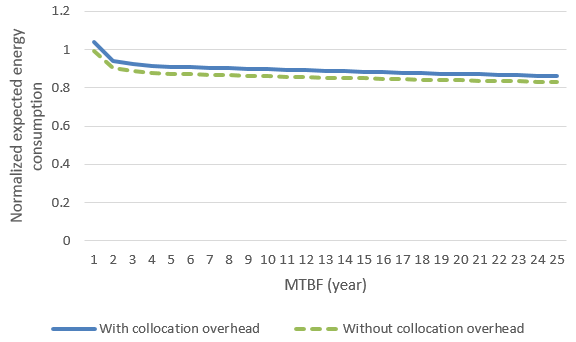
\includegraphics[width=\columnwidth]{Figures/collocation}
	\end{center}
	%\vskip -0.22in 
	\caption{Impact of collocation overhead on normalized energy consumption. $W=10^6$ hours, $N=10^6$, $\rho$=0.5, $\alpha$=5.}
	\label{fig:comp_vary_fail_speed}
\end{figure}